\chapter{The Internet Of Things}
\label{sec:background}

The Internet of Things (IoT) is a paradigm to which we put more and more attention in the scientific community.
But, what we understand as \textit{Internet of Things}?.

Some organizations\footnote{IEEE, towards an IoT definition http://goo.gl/u4AjEd} are trying to give a complete definition to this, but it still hard to have a common consensus.
However, for this thesis I will adopt a definition from my experience and my own understanding, also based in those definitions.
Since many protocols \textit{for} the Internet of Things exists, I will name those I used during my PhD, in order to explain an IoT infrastructure based in examples and experience.

\section{Towards an infrastructure for IoT}
An IoT infrastructure can be defined as a set of interconnected objects that use one or more different \textit{\textbf{current}} Internet protocols, in order to exchange information about the tasks for which they were programmed.
I highlight \textit{current} because interoperability between objects is easier to achieve using the Internet infrastructure that already exists.
However, the objects participating into this new infrastructure could be able or not to run the existing Internet protocols implementations, since the available hardware resources can vary from an object to another.
The choice of the hardware is driven by the use we make of it, since the application could require an specific placement and connectivity.
The usage of this objects can be very varied, from common sensing/actuating tasks (temperature, humidity, air quality, HVAC, access control) to small algorithms that provide basic functionalities, such as thermostats, coffee machines, traffic monitors, and so on.
For instance, objects used for environmental sensing applications often need to be installed at a specific place, which can be hard to reach. 
This forces to either reach the sensors with a specific cable, for both power and connectivity, or use wireless communications.
On the other hand, for other devices like home appliances or smart meters, the placement is often already defined, and they can be easily connected to an existing network.
For the first kind of applications mentioned above, wireless communications seems to be very convenient, while in the second example, a wired connection can already exist or could be easy to provide.
The communication method can determine the way we power the device, either using batteries or the electricity network.
Thus, two kind of objects with different hardware capabilities are present in an IoT infrastructure, which we can separate into constrained and non-constrained.
Non-constrained devices are often able to run modern implementations of Internet protocols, since the hardware capabilities provided by objects powered by the electricity network are usually high.
This also increase the cost of this objects, which avoid the use of them in applications where big quantities are needed.
Constrained devices, which are battery powered, does not provide enough computational resources to implement current Internet protocols \textit{as is}.
However, they can provide more flexibility of installation, due to their physical size and cost.

\subsection{Very constrained resources: a scientific challenge}
The computational resources such as memory, can vary from a tens of bytes for low-cost microcontroller (MCU) based objects, to hundreds or thousands of mega bytes in both ROM and RAM for System on a Chip (SoC) based objects, which are more expensive.
The very low-cost of MCU based objects, coupled with their very low-power capabilities, make them very easy to produce and could be spread in most of physical environments, such as forests, streets, buildings and homes, since it is possible to make them run in batteries.
We can call this objects \textit{\textbf{smart objects}}.
In this thesis, I will put emphasis on MCU based smart objects, since most of the scientific challenges come with the constrained resources in memory and energy of such devices.

\subsection{Communication between smart objects}
Several communication protocols are used in the current Internet.
Most of them are based on Ethernet, in which a standard cable is needed for each participant in the network.
A wireless Ethernet protocol was also standardized, as known as IEEE 802.11, providing the same features without the need of cables.
Other ways to reach the current Internet also exists, such as optical fiber, satellite and different radio standards, just to name a few.
Since the IoT aims to be ubiquitous, communication using cables would complicate the physical installation of such objects.
An advantage of MCU based objects is the very low power consumption.
Thus, a very low power communication interface would allow this objects to be powered using batteries.
Therefore, wireless communication protocols seem to be the best choice.
However, communication interfaces implementing standards like IEEE 802.11 were not built having low power features in mind, making them too inefficient if batteries are used as power source.
Several wireless devices manufacturers and research institutes worked together to create new energy-aware protocols to provide wireless communication for smart objects.
One of the standards that came from these efforts was the IEEE 802.15.4.
It was created specifically for low-power transceivers, allowing communication ranges near to 802.11, but offering a very low bandwidth.
This limitation avoid the exchange of large data packets, which also limits the protocols that can be managed by the interface, before having considerable fragmentation.
This memory constraints avoid the use of classical approaches to develop software for Internet based applications, often written in high level programming languages.
These approaches make use of common Internet protocol's implementations, which are not aware of this low resources.
Thus, a new way to provide Internet functionalities must be developed.
In 2003, Adam Dunkels developed a very lightweight TCP/IP protocol stack, uIP\cite{dunkels03full}, for 8-bit microcontrollers, giving a way to smart objects to communicate using a standard Internet protocol.
With this contribution, several services could be developed to create a first IoT infrastructure.
However, most of the services provided in Internet does not use a simple way to communicate, such as TCP/IP.
Therefore, a more complete framework for Internet services development should be created, to establish a more transparent and easy to use approach in resource constrained devices.

\subsection{6loWPAN, or how to give an IP address to any object}
With the arrival of the IPv6 standard\cite{rfc2460}, which enabled a wider range of IP addresses than the previous IPv4, the possibility to assign an address to each smart object became a reality.
This arise new challenges in the implementation for this new network protocol, since the RFC specification was intended for high resources machines.
Montenegro et al. proposed a new specification\cite{rfc4944} for constrained resources devices in order to communicate using IPv6 addresses.
This specification, called 6loWPAN (IPv6 for low-power Wireless Personal Area Networks) was successfully implemented\cite{durvy08making} and was able to provide interoperability with IPv6 ready devices, as it fulfill all the requirements to have an IPv6 label\footnote{https://www.ipv6ready.org/}.
In this way, we have a first real \textit{"Internet of Things"} where every smart object can be reached from anywhere on Internet.
With this, we can think about web services, since the objects themselves can already be part of a network where they can offer their embedded services, hosted in their small amount of memory.
A new way to represent this services is then required, that could meet the current web services specifications and approaches.

\subsection{An application layer for smart objects}
In the current Internet, web services are very often represented using the HTTP application protocol, in an architectural style called REST, defined by Fielding and Taylor\cite{Fielding02REST}.
REST services are very useful in the web, since they have a very easy way to operate using simple verbs: GET, POST, PUT, DELETE, just to name the common ones.
This representation could be very useful for smart objects, allowing the user, or other smart objects, to access its services in a standard way, providing interoperability with a good abstraction level.
An implementation of HTTP can be done for smart objects, but it takes a huge amount of memory in both RAM and ROM, being too heavy and inefficient for implementation on constrained, battery-powered devices\cite{Shelby10EWS}.
To solve this problem, Shelby et al. standardized the "HTTP for resource constrained devices"\cite{rfc7252}, called CoAP (Constrained Application Protocol).
This new application protocol is able to manage the methods described above, fulfilling the requirements for a RESTful API.
The services provided by the smart objects can be represented in a HTTP like form, i.e. \texttt{/sensors/temperature} for a temperature resource. If we use the CoAP command GET for this resource, we should have a response similar to "22.5", as an example of resource representation.
With a PUT or POST command in a resource, we can change their state in a physical way.
For instance, if we want to change the state of a LED, we access the resource \texttt{/leds} with a query \texttt{?color=red} for a red LED, and a payload \texttt{mode=on} in order to turn it on.
This API facilitates the exchange of information between other smart objects, as known as "Machine to Machine (M2M)" communication.
CoAP was also developed having in mind the interoperability issue that comes when we need to communicate with other machines, which don't use CoAP as application protocol, providing an easy way to translate the messages to HTTP.

\subsection{A comparison between protocols}
Having described a smart object capacities and capabilities, we can now make a layered comparison between a typical Internet and an IoT protocols suites, built from the protocols already mentioned above.

\begin{figure}[htb]
	\centering
	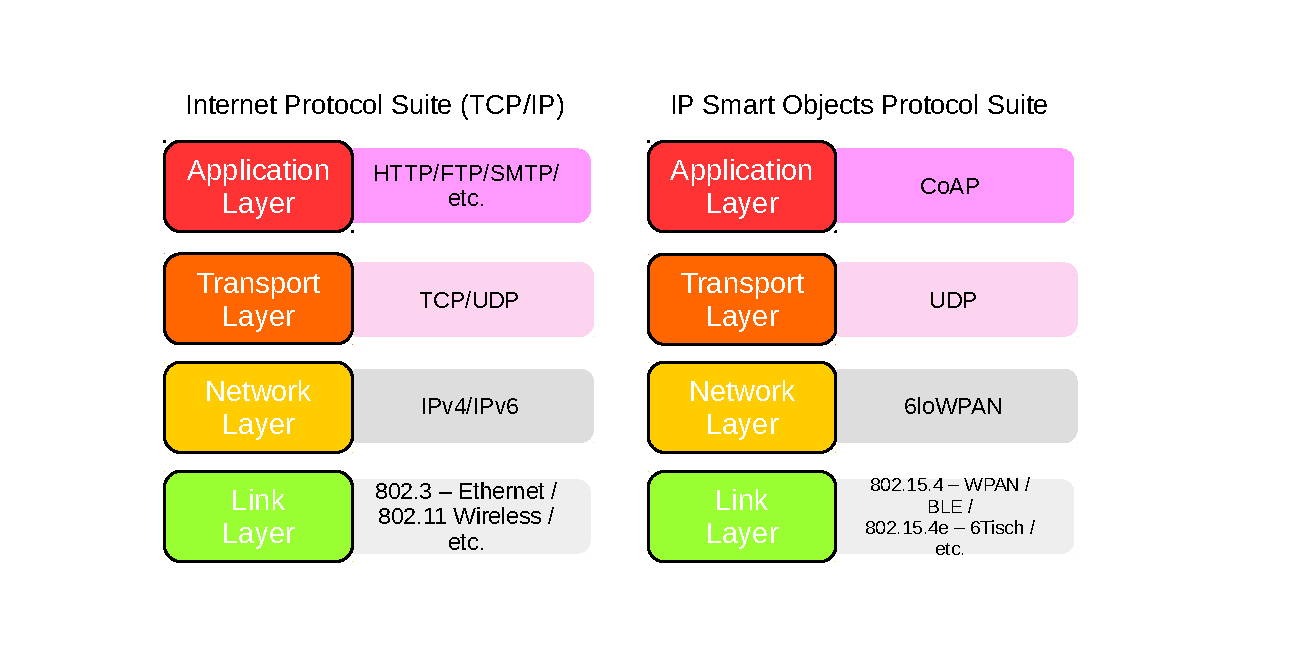
\includegraphics[width=0.95\columnwidth]{chapters/background.images/Layers.pdf}
	\caption{Comparison between Internet protocols}
	\label{fig:IPLayers}
\end{figure}

In figure \ref{fig:IPLayers} we can appreciate a layered representation of both suites, the traditional Internet and the IoT.


\todo{introduce contiki and other OS}

\todo{options to update firmware}

\todo{firmware update management tools}